\documentclass[tikz,border=4pt]{standalone}
\usepackage{amsmath}
\usetikzlibrary{arrows.meta,decorations.pathmorphing}
\definecolor{marked}{RGB}{38,91,151}
\tikzset{vertex/.style={circle,fill=black,inner sep=1.3pt},insertion/.style={rectangle,draw,fill=white,inner sep=2pt},prop/.style={decorate,decoration={coil,aspect=.65,segment length=4mm,amplitude=1.1mm},line width=.45pt}}
\newcommand{\edge}[2]{\draw[prop] (#1)--(#2);\draw[-{Stealth[length=1.5mm]},line width=.5pt] ($(#1)!.45!(#2)$)--($(#1)!.56!(#2)$);}
\usetikzlibrary{calc}
\begin{document}
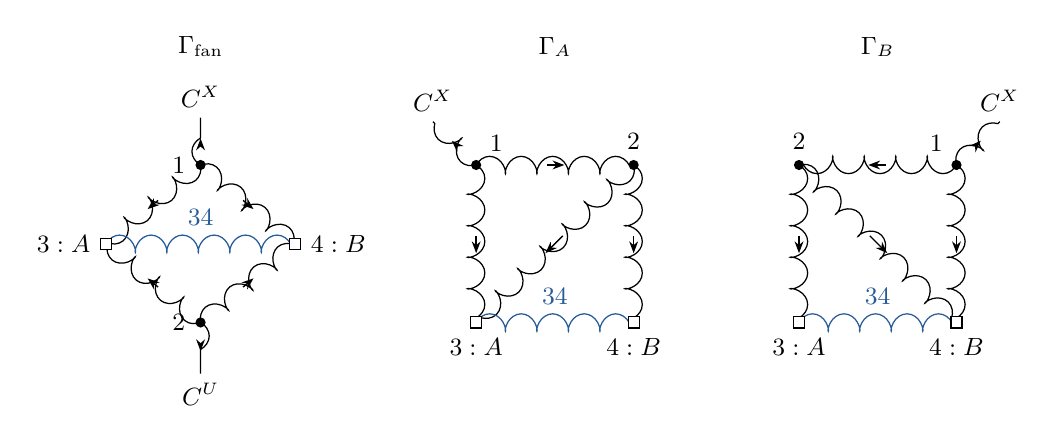
\begin{tikzpicture}[x=1cm,y=1cm,font=\small]
\begin{scope}
\node at (1.2,4){$\Gamma_{\mathrm{fan}}$};
\coordinate (a) at (1.2,2.5);\coordinate (b) at (1.2,.5);\coordinate (A) at (0,1.5);\coordinate (B) at (2.4,1.5);
\edge{a}{A}\edge{a}{B}\edge{b}{A}\edge{b}{B}
\draw[prop,marked] (A)--(B) node[midway,above=3pt] {$34$};
\coordinate (x) at (1.2,3.1);\coordinate (u) at (1.2,-.15);\edge{a}{x}\edge{b}{u}
\node[vertex,label=left:$1$] at (a){};\node[vertex,label=left:$2$] at (b){};
\node[insertion,label=left:$3:A$] at (A){};\node[insertion,label=right:$4:B$] at (B){};
\node[above] at (x){$C^X$};\node[below] at (u){$C^U$};
\end{scope}
\begin{scope}[xshift=4.5cm]
\node at (1.2,4){$\Gamma_A$};
\coordinate (a) at (.2,2.5);\coordinate (b) at (2.2,2.5);\coordinate (A) at (.2,.5);\coordinate (B) at (2.2,.5);
\edge{a}{b}\edge{a}{A}\edge{b}{A}\edge{b}{B}
\draw[prop,marked] (A)--(B) node[midway,above=3pt] {$34$};
\coordinate (x) at (-.35,3.05);\edge{a}{x}\node[above] at (x){$C^X$};
\node[vertex,label=above right:$1$] at (a){};\node[vertex,label=above:$2$] at (b){};
\node[insertion,label=below:$3:A$] at (A){};\node[insertion,label=below:$4:B$] at (B){};
\end{scope}
\begin{scope}[xshift=8.6cm]
\node at (1.2,4){$\Gamma_B$};
\coordinate (a) at (2.2,2.5);\coordinate (b) at (.2,2.5);\coordinate (A) at (.2,.5);\coordinate (B) at (2.2,.5);
\edge{a}{b}\edge{a}{B}\edge{b}{A}\edge{b}{B}
\draw[prop,marked] (A)--(B) node[midway,above=3pt] {$34$};
\coordinate (x) at (2.75,3.05);\edge{a}{x}\node[above] at (x){$C^X$};
\node[vertex,label=above left:$1$] at (a){};\node[vertex,label=above:$2$] at (b){};
\node[insertion,label=below:$3:A$] at (A){};\node[insertion,label=below:$4:B$] at (B){};
\end{scope}
\end{tikzpicture}
\end{document}
